\documentclass[12pt, usepdftitle=false]{beamer}
\usetheme{Singapore}  %% Themenwahl
\usecolortheme{myct}
\usepackage{color}
\usepackage{graphicx}
\usepackage{ragged2e}
\usepackage[defaultsans]{droidsans}
\usepackage{hyperref}
\usepackage{amssymb}% http://ctan.org/pkg/amssymb
\usepackage{pifont}% http://ctan.org/pkg/pifont
\usepackage[T1]{fontenc}
\usepackage{hyperref}
\newcommand{\cmark}{\textcolor{green}{\ding{51}}}%
\newcommand{\xmark}{\textcolor{red}{\ding{55}}}%
 
\newcommand{\backupbegin}{
   \newcounter{finalframe}
   \setcounter{finalframe}{\value{framenumber}}
}
\newcommand{\backupend}{
   \setcounter{framenumber}{\value{finalframe}}
}

\graphicspath{{./images/}}

\title[Bitcoin]{Guest Lecture: An Introduction to \vspace*{1em}}
\subtitle{
\includegraphics[width=5cm]{btcLogo}}

\logo{
\includegraphics[width=.05\textwidth]{logo-grey.pdf}}

\author{Murch}
\date{2015-06-02}

\hypersetup{pdfinfo={
	Title=An Introduction to Bitcoin,
	Author=Murch,
	}
}
 
\begin{document}
\frame[plain]{\titlepage}

\frame{\tableofcontents}

\section{Introduction}
\frame{\tableofcontents[currentsection]}

\begin{frame}{Who am I?}
\begin{columns}[c]
\begin{column}{.7\textwidth}
	\begin{description}[leftmargin=0em]
		\item[Name:] Murch
		\item[Job:] my job 
		\item[Why here?] Because I can't stop talking and thinking about Bitcoin
		\item[Qualification:] Spent lots of time reading and writing about Bitcoin
	\end{description}
\end{column}
\begin{column}{.3\textwidth}
\only<1->{
\includegraphics[width=.8\textwidth]{ME}}
\end{column}
\end{columns}
\end{frame}

%%-------------------------------------------------------------------------------------------------------------

\section{What is Money?}
\frame{\tableofcontents[currentsection]}
\begin{frame}{What is money?}

\begin{center}
\vspace{1em}
Examples for Money?\pause
\vspace{1em}

Properties of Money?
\end{center}

\end{frame}

\begin{frame}<1,2>[label=def]{\only<3>{\alert{Review: }} Definition of Money}
\begin{definition} 
Money is any object or verifiable record that is generally accepted as payment for goods and services and repayment of debts in a given socio-economic context or country.

The main functions of money are distinguished as:
\begin{itemize}
	\item medium of exchange
	\item unit of account
	\item store of value 
\end{itemize}
	\begin{flushright}
	\tiny{Definition [en.wikipedia.org/wiki/Money]}
	\end{flushright}%
\end{definition}%
\vspace{.5em}%
\only<1>{~ ~}\only<2>{Money is a technology that facilitates trade.}

\end{frame}

%%-------------------------------------------------------------------------------------------------------------

\begin{frame}{Two Categories of Money} 
\pause
		\begin{definition}
		\emph{Commodity Money} is based on the inherent value of the exchange medium.
		\end{definition}
		Examples: \pause Gold 
\includegraphics[width=.05\textwidth]{commodity.pdf}, Shells 
\includegraphics[width=.04\textwidth]{shells.pdf}, Cigarettes 
\includegraphics[width=.05\textwidth]{cigarettes.pdf}, Livestock
	\vspace{1em}
\pause

		\begin{definition}
		\emph{Fiat Money} is inherently worthless, but derives value from being a promisory note issued by a nation or company.
		\end{definition}
		Examples: \pause US Dollar 
\includegraphics[width=.07\textwidth]{dollar.pdf}, Euro 
\includegraphics[width=.07\textwidth]{euro.pdf}, Bank statement
\end{frame}

%%-------------------------------------------------------------------------------------------------------------

\begin{frame}{What shortfalls does Money have?}

	\begin{center}
		So, Money is pretty useful, but... \pause
	\vspace{1em}

		\alert{What problems can you think of?}
	\end{center}

\end{frame}

\begin{frame}{Currency is inefficient and slow}
	\begin{itemize}
		\item Wire transfers take 2+ days
		\item Intercontinental wire transfers 7+ days
		\item Handling cash is inconvenient
	\end{itemize}
\end{frame}

%%-------------------------------------------------------------------------------------------------------------

\begin{frame}{Currency is expensive to maintain}
	\begin{itemize}
		\item Cash has to be counted and transported
		\item Bills have to be replaced every 2-5 years
		\item After time coins' value lower than production cost
	\end{itemize}
\end{frame}

%%-------------------------------------------------------------------------------------------------------------

\begin{frame}{Digital currency lacks privacy}

	\begin{itemize}
		\item Bank tracks your payments
		\item Credit Card Companies track your payments
		\item Government tracks your payments
	\end{itemize}

	Only cash is private.
\end{frame}

%%-------------------------------------------------------------------------------------------------------------

\begin{frame}{Inflation}
	\begin{itemize}
		\item Goverments set money policy
		\item Banks create additional money
	\end{itemize}
\end{frame}

%%-------------------------------------------------------------------------------------------------------------

\begin{frame}{Loss of Purchasing Power}
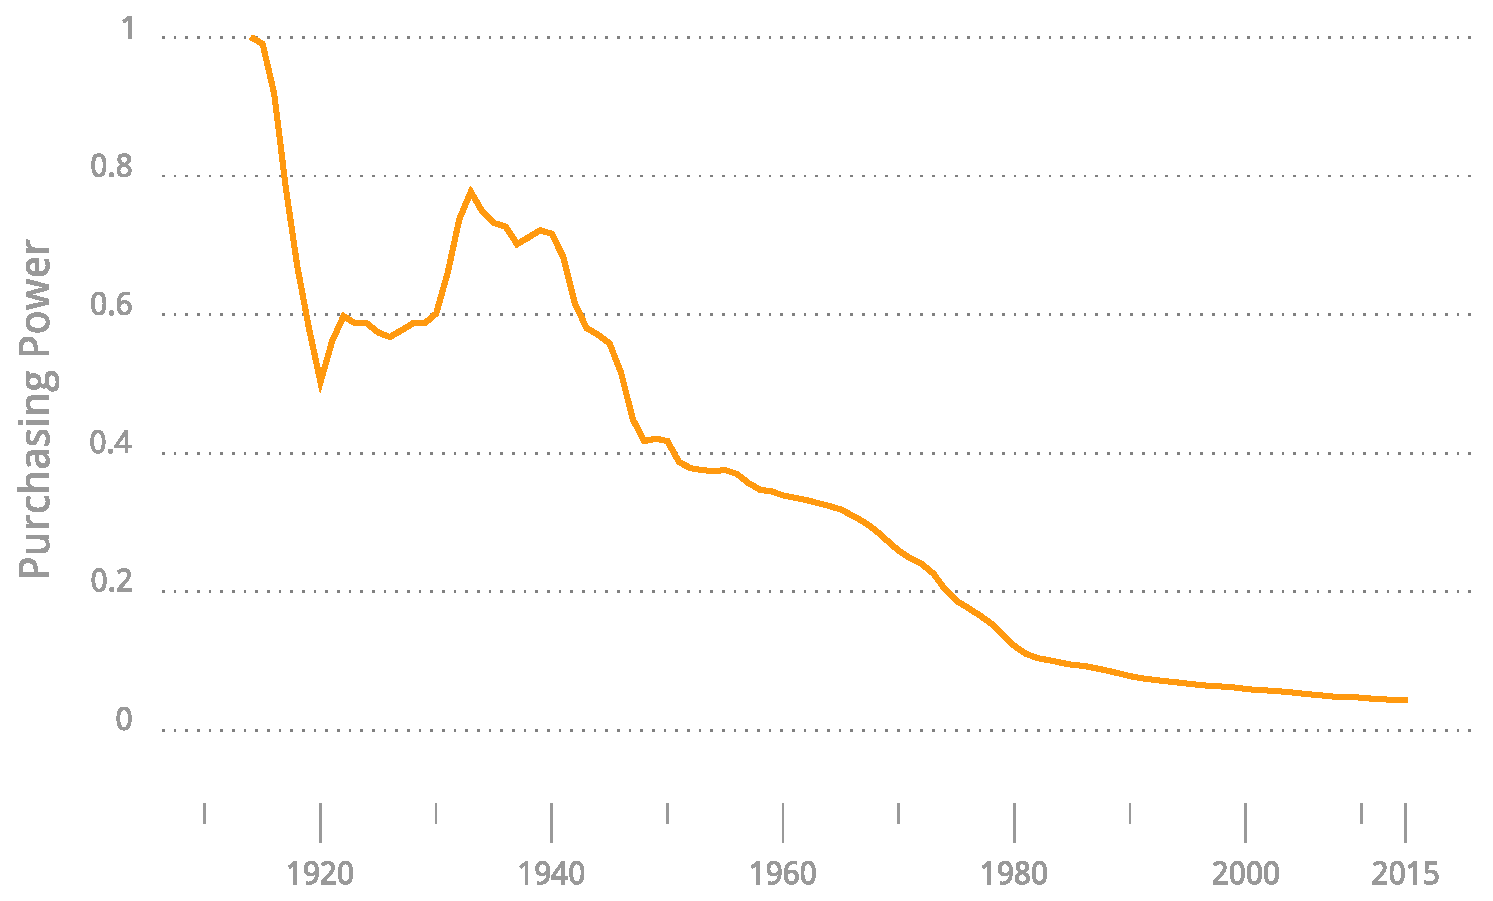
\includegraphics[width=\textwidth]{cpi.pdf}
	\begin{flushright}
	\tiny{Data: U.S. Bureau of Labor Statistics, Detailed CPI report 2015-04}
	\end{flushright}
\end{frame}

%%-------------------------------------------------------------------------------------------------------------

\begin{frame}{Lack of Control}
	\begin{itemize}
		\item Transfer and Storage controlled by third parties
		\item Limited Freedom to choose recipients
		\item Counter-party risk
	\end{itemize}
\end{frame}

%%-------------------------------------------------------------------------------------------------------------
%%-------------------------------------------------------------------------------------------------------------

\section{What is Bitcoin?}
\frame{\tableofcontents[currentsection]}

%%-------------------------------------------------------------------------------------------------------------

\begin{frame}{What is the connection to Bitcoin?}

	Bitcoin is a new payment system designed to address these problems.
	
\end{frame}

\begin{frame}{Enter Satoshi Nakamoto}

\begin{center}
\includegraphics<1>[width=.5\textwidth]{satoshi.pdf}
%% \includegraphics<2>[width=.5\textwidth]{satoshi2.pdf}
\end{center}
	
\end{frame}

%%-------------------------------------------------------------------------------------------------------------

\begin{frame}{Bitcoin in a nutshell}
\begin{columns}[c]
\begin{column}{.3\textwidth}

\includegraphics[width=\textwidth]{logo-grey}
\end{column}
\begin{column}{.7\textwidth}
\begin{itemize}
	\item New way to send payments via internet\pause
	\item Agreement to treat digital tokens named \alert{bitcoins} as money\pause
	\item Digital cash: irreversible and no middlemen\pause
	\item All transactions are publicly visible\pause
	\item Users remain private
\end{itemize}
\end{column}
\end{columns}
\end{frame}

%%-------------------------------------------------------------------------------------------------------------

\begin{frame}{Privacy in Bitcoin}
\begin{center}
	\only<1>{
\includegraphics[width=.5\textwidth]{privacy1.pdf}}%
	\only<2>{
\includegraphics[width=.5\textwidth]{privacy2.pdf}}%
\end{center}
\end{frame}

%%-------------------------------------------------------------------------------------------------------------

\begin{frame}{Spending bitcoins}
\begin{center}
	\only<1>{
\includegraphics[width=.7\textwidth]{transaction1.pdf}}%
	\only<2>{
\includegraphics[width=.7\textwidth]{transaction2.pdf}}%
	\only<3>{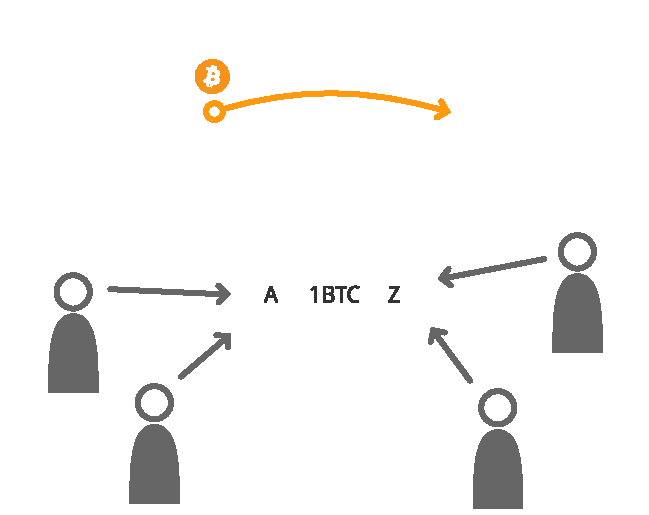
\includegraphics[width=.7\textwidth]{transaction3.pdf}}%
	\only<4>{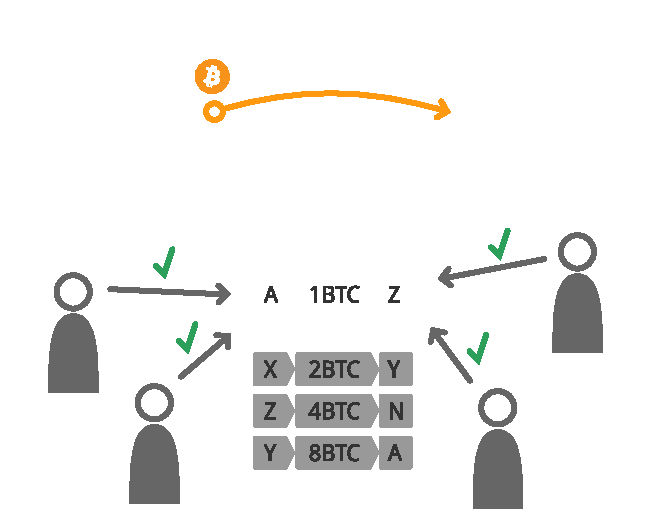
\includegraphics[width=.7\textwidth]{transaction4.pdf}}%
	\only<5>{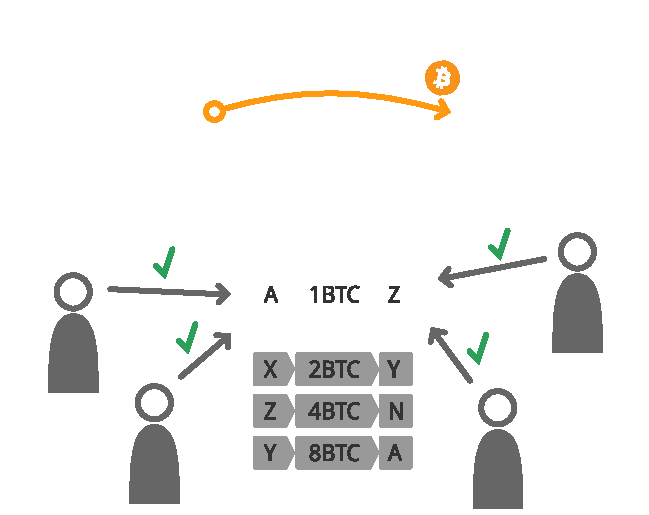
\includegraphics[width=.7\textwidth]{transaction5.pdf}}%
\end{center}
\end{frame}

%%-------------------------------------------------------------------------------------------------------------

\begin{frame}{Let's see this live}
	
	\begin{center}
	
\includegraphics[width=.4\textwidth]{pubkey.png}

\vspace{1em}
Address: \href{https://blockchain.info/address/1LNHme4E5mrhUk4tbLpb75Q5aq81F8Mb95}{1LNHme4E5mrhUk4tbLpb75Q5aq81F8Mb95}
	\end{center}
\end{frame}

%%-------------------------------------------------------------------------------------------------------------


\begin{frame}{Who pays for Bitcoin?}
\begin{center}
	\only<1>{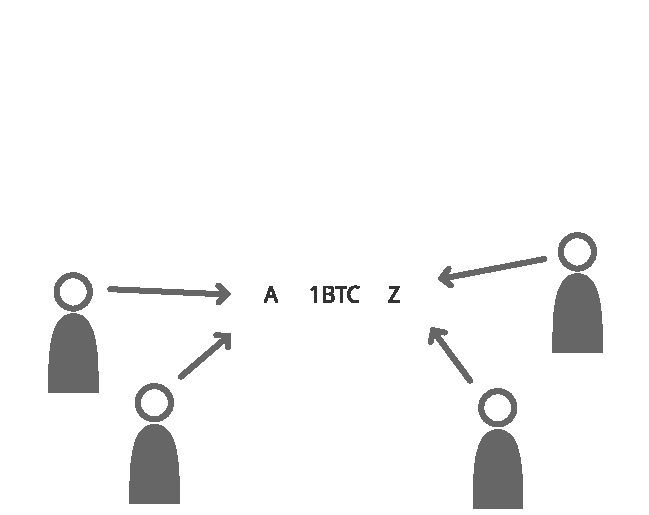
\includegraphics[width=.7\textwidth]{financing1.pdf}}%
	\only<2>{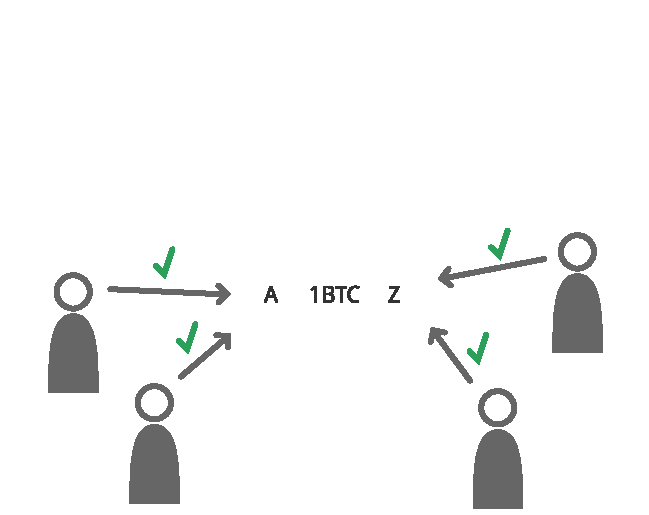
\includegraphics[width=.7\textwidth]{financing2.pdf}}%
	\only<3>{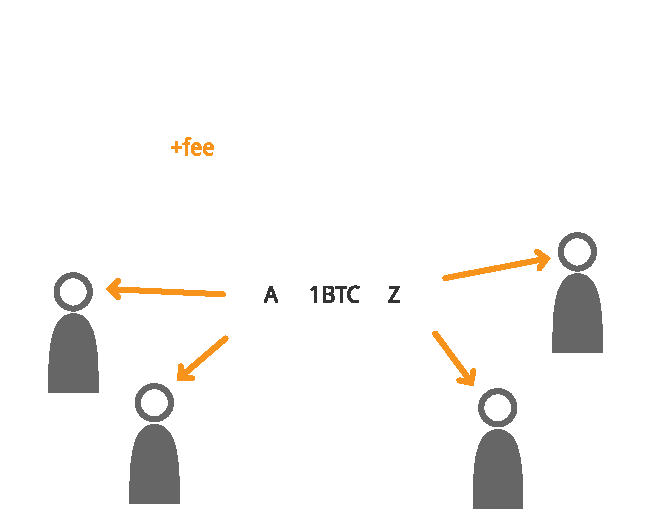
\includegraphics[width=.7\textwidth]{financing3.pdf}}%
	\only<4>{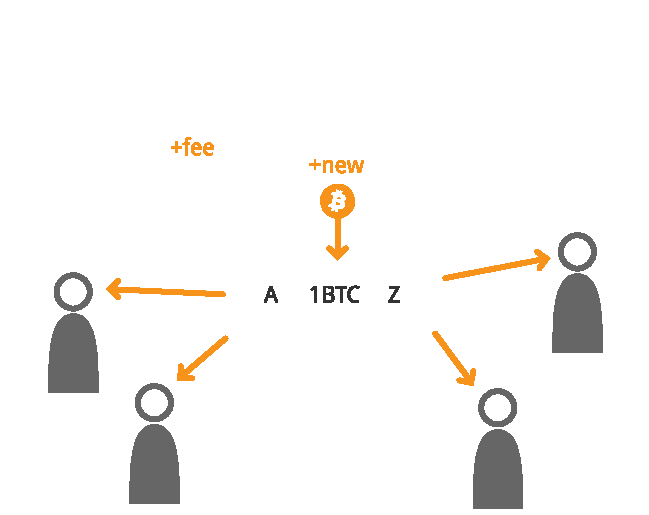
\includegraphics[width=.7\textwidth]{financing4.pdf}}%
	\only<5>{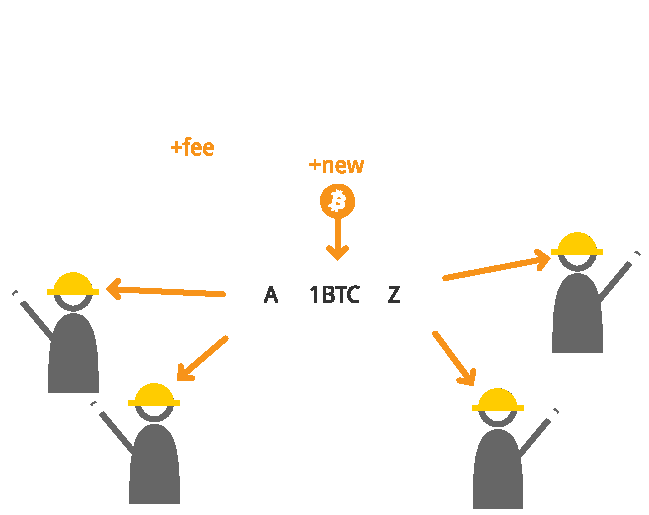
\includegraphics[width=.7\textwidth]{financing5.pdf}}%
\end{center}
\end{frame}

%%-------------------------------------------------------------------------------------------------------------

\begin{frame}{Bitcoin is a Limited Resource}
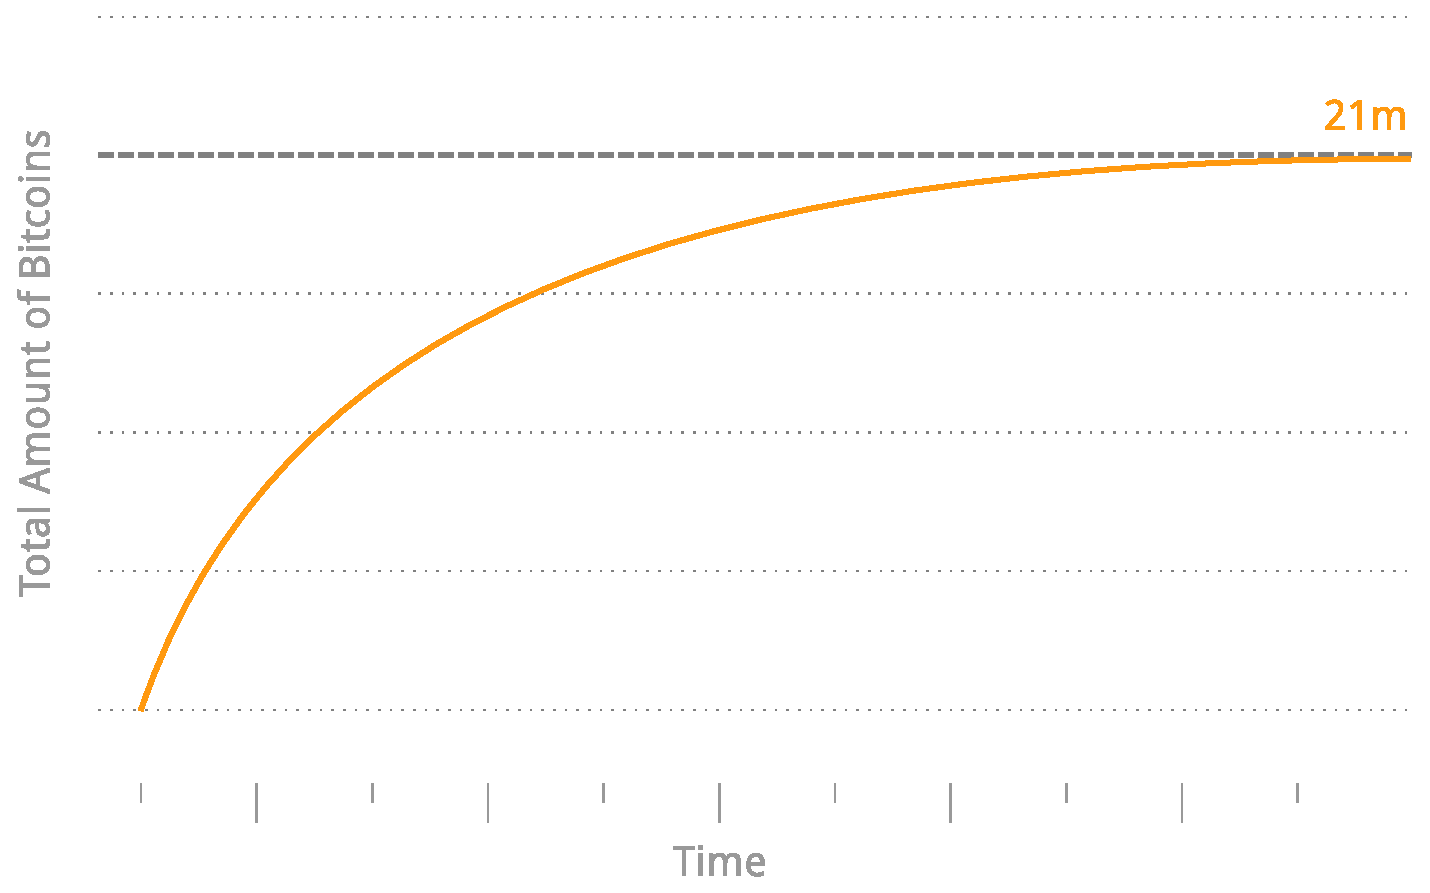
\includegraphics[width=\textwidth]{scarcity.pdf}

\end{frame}

%%-------------------------------------------------------------------------------------------------------------

\begin{frame}{Getting started with Bitcoin}
\begin{enumerate}
\pause\item Inform yourself: \alert{bitcoin.org}
\pause\item Get a wallet
\begin{description}
\item[Desktop] 
\includegraphics[height=1em]{multibit} MultiBit
\item[Android] 
\includegraphics[height=1em]{bitcoinwallet}  Bitcoin Wallet
\item[iOS] 
\includegraphics[height=1em]{breadwallet}  breadwallet
\end{description}
\pause\item{Get bitcoins}
\pause\item{Spend bitcoins}
\end{enumerate}
\end{frame}

%%-------------------------------------------------------------------------------------------------------------

\begin{frame}{That's how Bitcoin works}
	
\begin{center}
	\only<1>{Any questions so far?}
	%%\only<2>{
\includegraphics[width=.4\textwidth]{privkey.png}\\
	%%The private key to the address from before}
\end{center}

\end{frame}

%%-------------------------------------------------------------------------------------------------------------
\againframe<3>{def}

\begin{frame}{Is Bitcoin Money?}
	\only<1->{\begin{itemize}
		\item Verifiable Record \only<3->{\cmark}
		\item Acceptance \only<4->{\cmark / \xmark}
		\item Medium of Exchange \only<5->{\cmark}
		\item Unit of Account \only<6->{\cmark}
		\item Store of Value  \only<7->{\cmark / \xmark}
	\end{itemize}}\pause

\emph{Bitcoin} is not \emph{legal tender}, but a complementary currency. It shares aspects of both \emph{commodity money} and \emph{fiat money}.

\end{frame}

%%-------------------------------------------------------------------------------------------------------------

\begin{frame}{Does Bitcoin solve other Moneys' shortfalls?}

\begin{table}[h]
	\begin{tabular}{ll}
\vspace{.5em}
\textbf{Issue} & \textbf{Bitcoin} \\
	Slow & Fast \\
	Expensive to maintain & Network pays for itself \\
	Lack of Privacy & Private/Pseudonymous \\
	Inflated & Limited Supply\\
	Lack of Control & Puts user in control
	\end{tabular}
\end{table}

\end{frame}

%%-------------------------------------------------------------------------------------------------------------

\begin{frame}{What makes bitcoins valuable?}

Bitcoin is a limited resource and useful/convenient.

\end{frame}

%%-------------------------------------------------------------------------------------------------------------

\begin{frame}{What are the downsides to Bitcoin?}
	\begin{itemize}
		\pause\item Responsibility
		\pause\item Limited Acceptance
		\pause\item Legal status to be determined
		\pause\item Volatility and no inherent value
		\pause\item Reputation
		%% TODO EAch its own slide
	\end{itemize}
\end{frame}

%%-------------------------------------------------------------------------------------------------------------

\section{History of Bitcoin}
\begin{frame}{A Brief History of Bitcoin}
	\vspace{0em}
	\only<1>{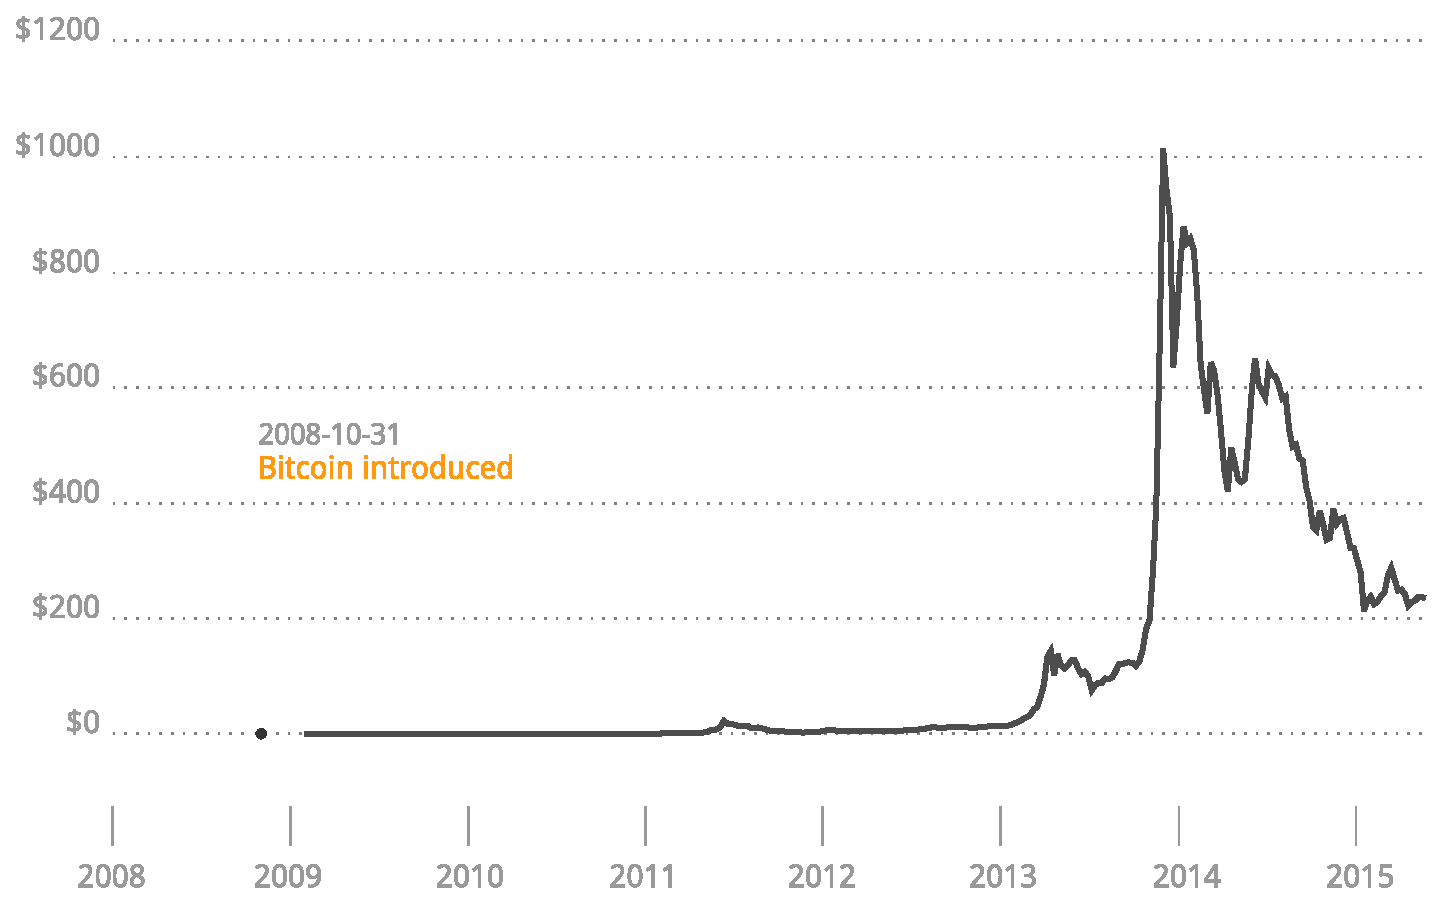
\includegraphics[width=\textwidth]{1.pdf}}%
	\only<2>{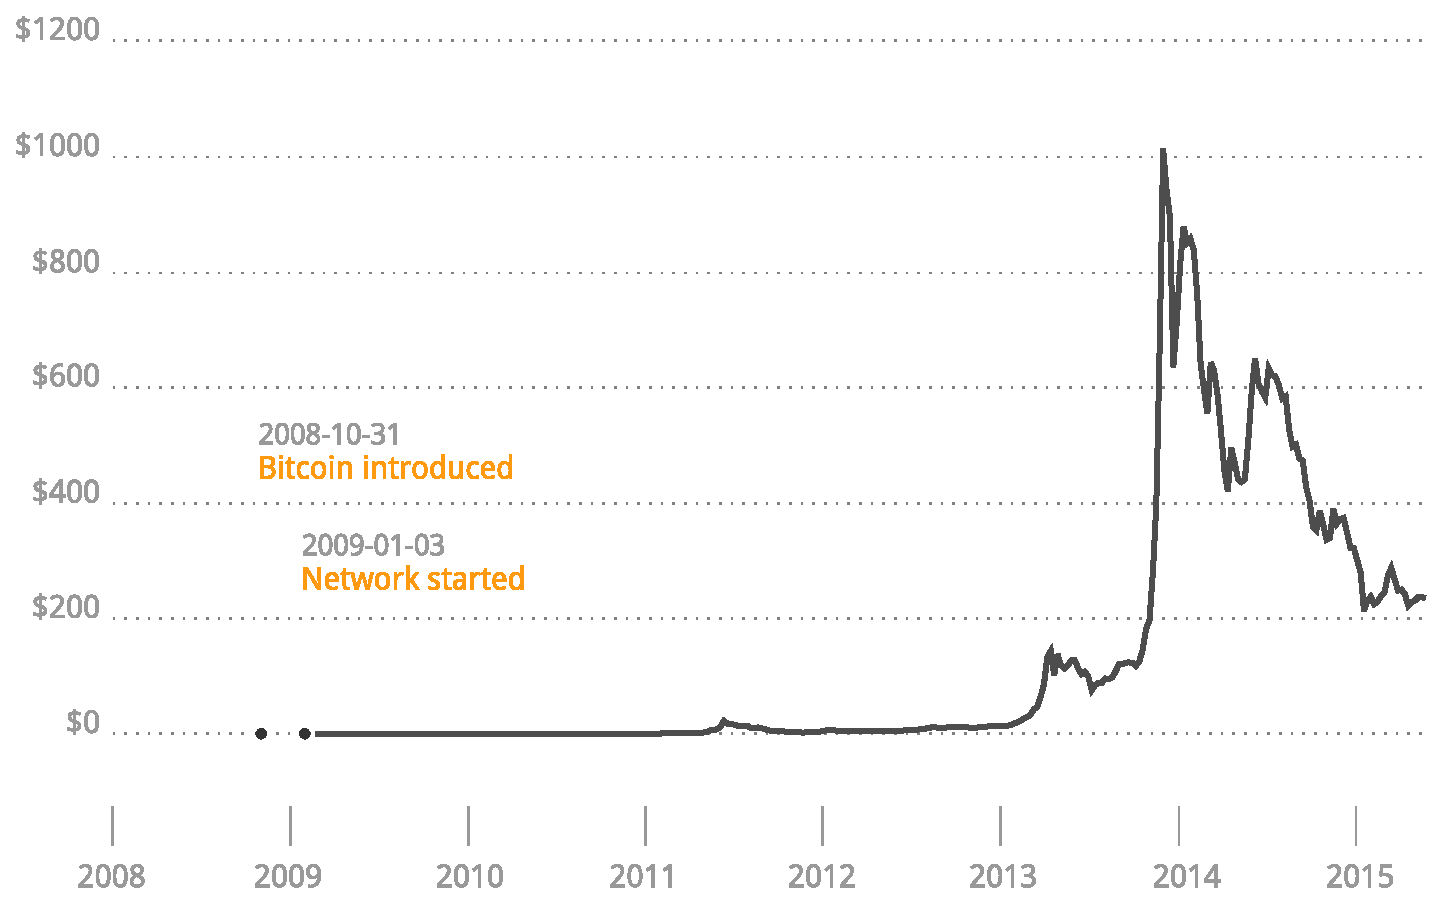
\includegraphics[width=\textwidth]{2.pdf}}%
	\only<3>{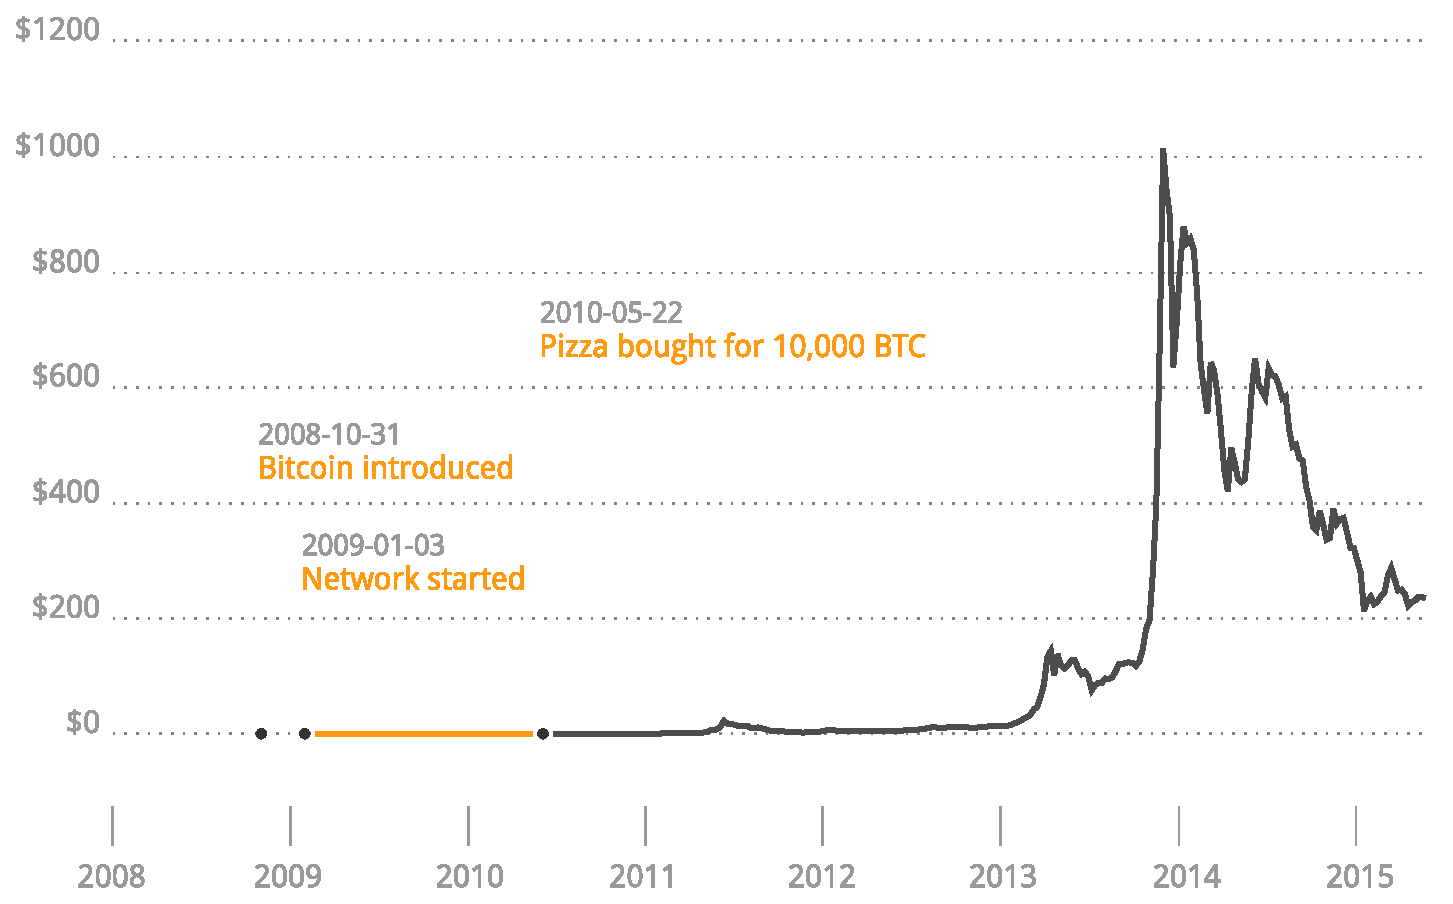
\includegraphics[width=\textwidth]{3.pdf}}%
	\only<4>{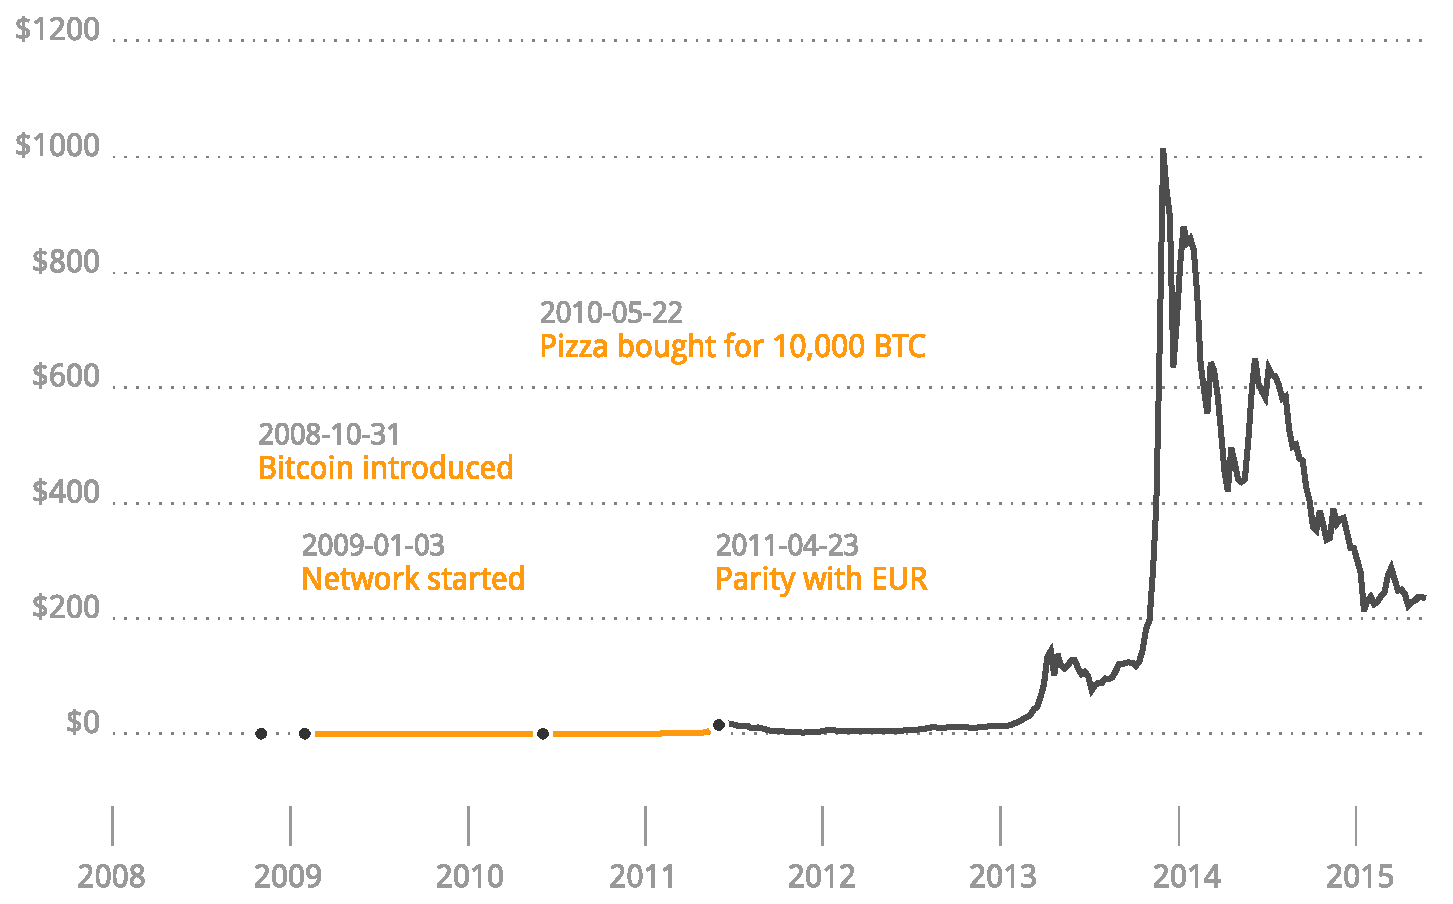
\includegraphics[width=\textwidth]{4.pdf}}%
	\only<5>{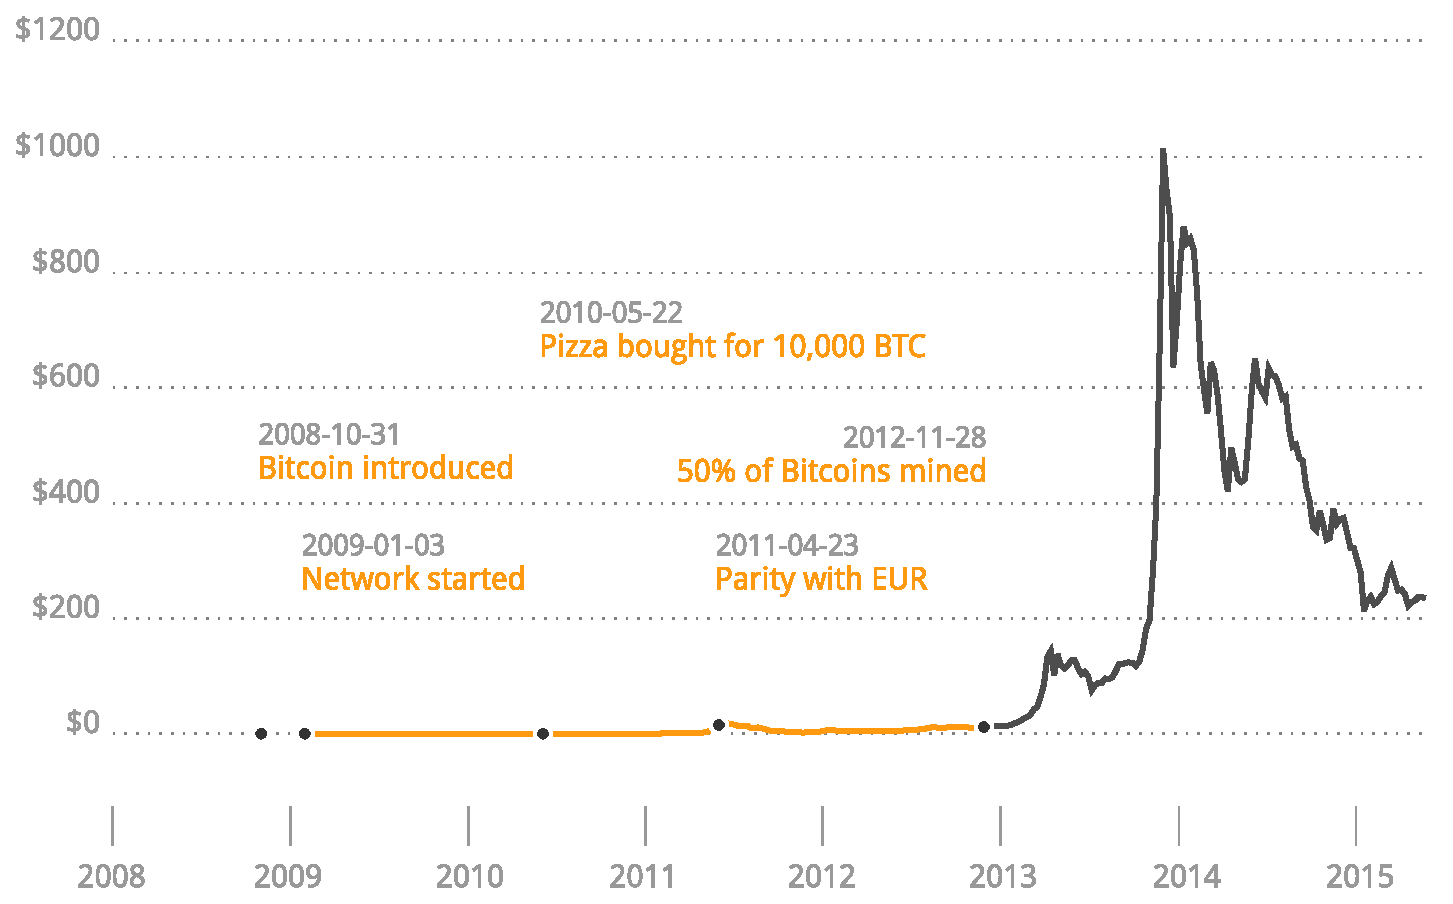
\includegraphics[width=\textwidth]{5.pdf}}%
	\only<6>{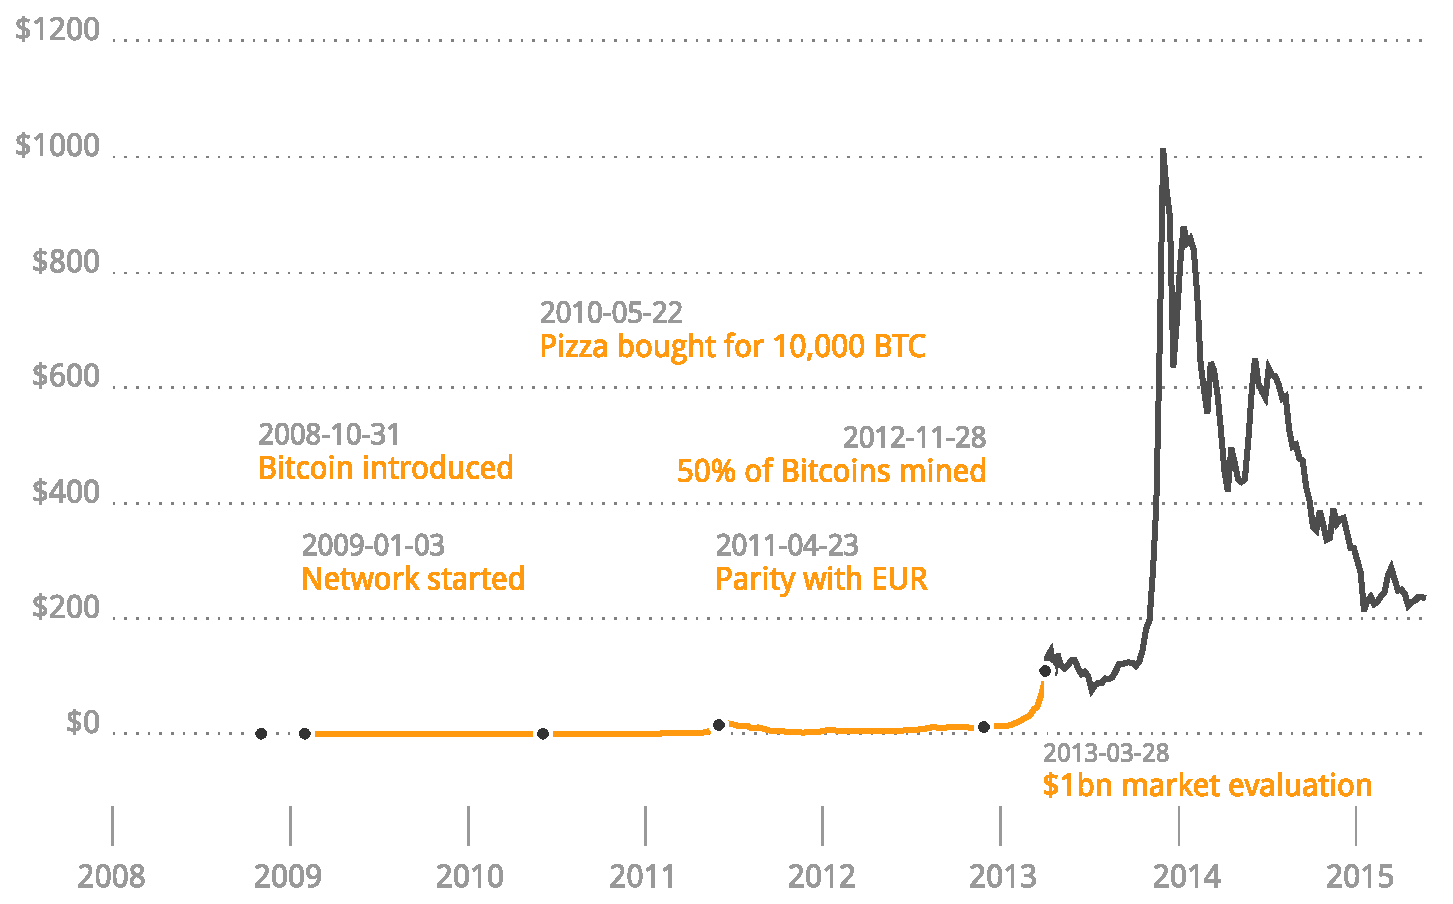
\includegraphics[width=\textwidth]{6.pdf}}%
	\only<7>{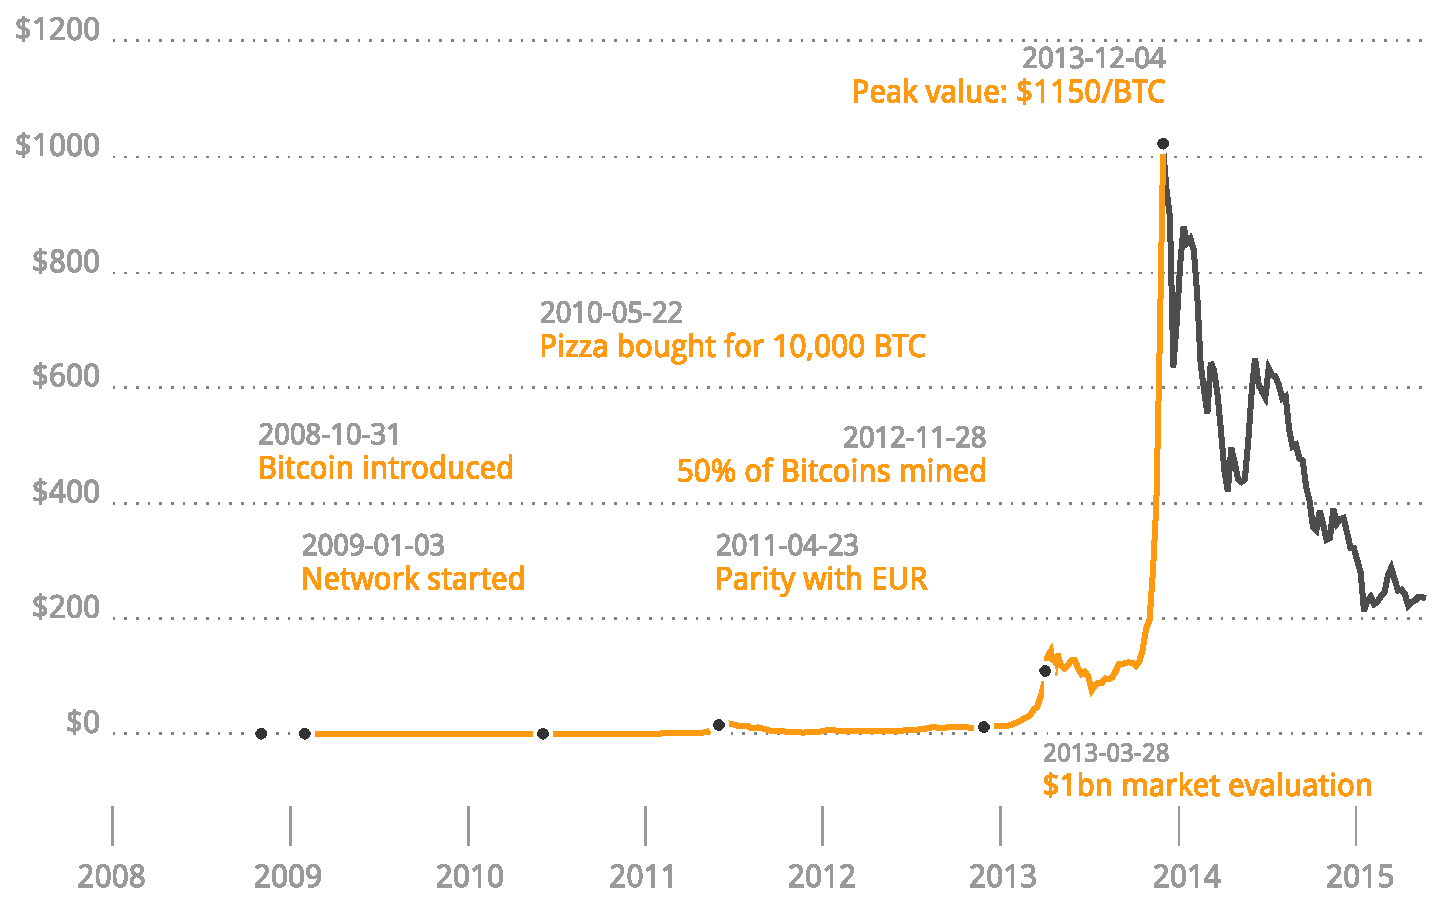
\includegraphics[width=\textwidth]{7.pdf}}%
	\only<8>{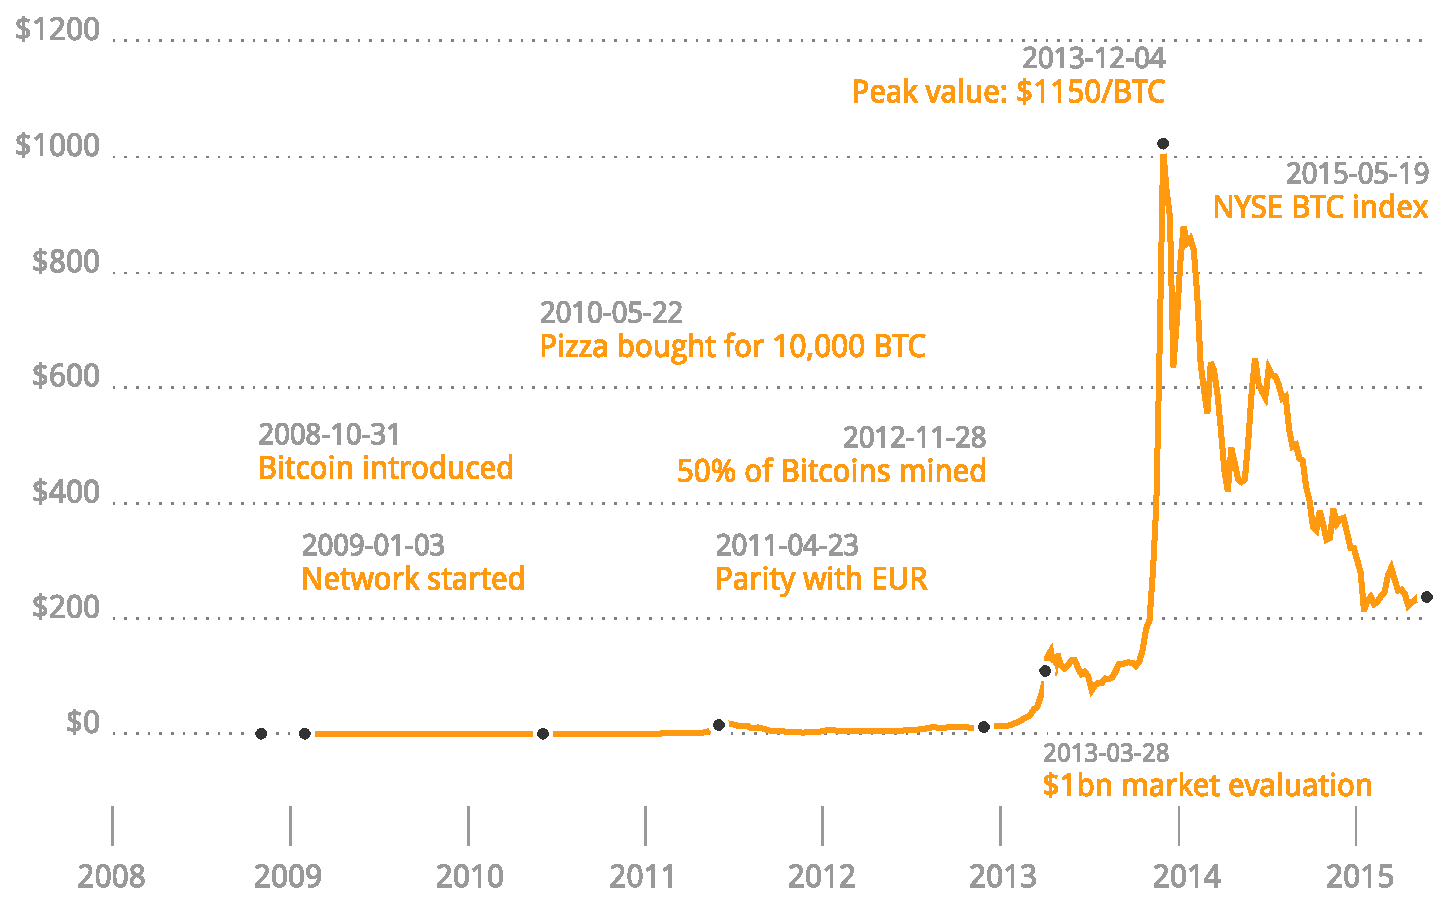
\includegraphics[width=\textwidth]{8.pdf}}%
	\begin{flushright}
	\tiny{Marketdata: [CoinDesk.com] | Events: [HistoryOfBitcoin.org]}
	\end{flushright}
\end{frame}

%%-------------------------------------------------------------------------------------------------------------

\begin{frame}{Bitcoin Today}
\begin{itemize}
	\pause\item Still experimental
	\pause\item Estimated Userbase: $\sim$500.000 - 2.000.000
	\pause\item Transactions per day: $\sim$110.000
	\pause\item Accepted by 100.000+ merchants, including Microsoft, Dell, Lieferservice.de
	\pause\item Regulation in progress
	\pause\item Altcoins: $\sim$725, e.g. 

\includegraphics[height=1em]{litecoin.png},~ 

\includegraphics[height=1em]{doge.png},~ 

\includegraphics[height=1em]{ripple-sm},~ 

\includegraphics[height=1em]{nxt.png},~ 

\includegraphics[height=1em]{dash.png}
\end{itemize}

\end{frame}

%%-------------------------------------------------------------------------------------------------------------
%%-------------------------------------------------------------------------------------------------------------
%%-------------------------------------------------------------------------------------------------------------

\begin{frame}{Thank you for your attention}

\begin{center}
	\pause

	Any more questions?
\end{center}
\end{frame}

%%-------------------------------------------------------------------------------------------------------------
%%-------------------------------------------------------------------------------------------------------------
%%-------------------------------------------------------------------------------------------------------------

\appendix
\backupbegin

\begin{frame}{Byzantine Generals' Problem}

	Bitcoin solves the \emph{Byzantine Generals' Problem}: How to achieve consensus in a distributed network with potential adversaries.
\end{frame}

%%-------------------------------------------------------------------------------------------------------------

\begin{frame}{Alternative Bitcoin Definition}
\begin{definition}
Bitcoin is a \alert<3>{payment protocol} that provides a \alert<4>{public ledger} maintained by a \alert<5>{decentral} \alert<6>{peer-to-peer network} \alert<7>{secured with cryptographic proof}.
\end{definition}\pause

\only<2>{... quite a mouthful, huh?}
\only<3->{What is most important about that is:}
\begin{itemize}
\item<3->It's open-source software.
\item<4->Very little trust required in other participants of the network.
\item<5->No one entity controls the network.
\item<6->Any user can send money directly to peers.
\item<7->Solves the double-spend problem, and counterfeiting.
\end{itemize}
\end{frame}

%%--------------------------------------------------------------------------------------------------------------

\begin{frame}{What makes bitcoins valuable?}
Bitcoin recombines some of the best features of \emph{Cash}, \emph{Credit Cards}, and \emph{Wire transfers}.
	\begin{description}
		\pause\item[Global] Anyone with an internet connection can use it.
		\pause\item[Fast] Visible within seconds, confirmed after minutes.
		\pause\item[Secure] Doesn't require you to reveal your secret to spend money.
		\pause\item[Scarce] Limited to 21 Million units.
		\pause\item[Peer-to-peer] Payments go directly from user to user.
		\pause\item[Cheap] Send any amount of money for less than one cent.
		\pause\item[Open] No consent required to use it.
	\end{description}\pause
	\begin{block}{Conclusion}
	As the Bitcoin network is useful, but not owned by any single entity, the built-in units encompass the value of the network. As the network grows in usefulness, one can expect the value to rise.
	\end{block}
\end{frame}

%%-------------------------------------------------------------------------------------------------------------

\begin{frame}{Detailed Comparison to other forms of Money}
\begin{table}[h]  
\centering
\resizebox{\columnwidth}{!}{%
\begin{tabular}{llll}
\hline
\textbf{Transaction Cost} & \textbf{Precious Metals} & \textbf{Fiat Currencies} & \textbf{Bitcoin}           \\ \hline
\textbf{Storage}          & 0.15\% to 1\% p.a.       & Subsidized by FRB        & Free                       \\
\textbf{Transportation}   & Expensive                & Inconvenient             & Easy \& Free               \\
\textbf{Fiduciary Media}  & Inevitable               & Inherent                 & Impossible                 \\
\textbf{Recordkeeping}    & Manual                   & Mostly manual		& Automatic                  \\
\textbf{Issuance}         & Mining                   & Politics                 & Algorithm                  \\
\textbf{Payment Clearing} & Expensive                & Centralized              & Cheap \& Distributed       \\
\textbf{Scarcity}         & High                     & Arbitrary                & Fixed - 21 million \\
\textbf{Authentication}   & Expensive Assay          & Trust counterparty       & Built-in                   \\
\textbf{Security}         & Physical                 & Institutional            & Cryptographic              \\ \hline
\end{tabular}
}
\end{table}

\end{frame}

%%-------------------------------------------------------------------------------------------------------------

\begin{frame}{Addresses in Detail}
\end{frame}

%%-------------------------------------------------------------------------------------------------------------

\begin{frame}{Transactions in Detail}
\end{frame}

%%-------------------------------------------------------------------------------------------------------------

\begin{frame}{Blocks in Detail}
\end{frame}

%%-------------------------------------------------------------------------------------------------------------

\begin{frame}{Private Keys in Detail}
\end{frame}

%%-------------------------------------------------------------------------------------------------------------

\begin{frame}{Transactions in Detail}
\end{frame}

%%-------------------------------------------------------------------------------------------------------------

\begin{frame}{Blockchain in Detail}
\end{frame}

%%-------------------------------------------------------------------------------------------------------------

\begin{frame}{Who controls Bitcoin?}
\end{frame}

%%-------------------------------------------------------------------------------------------------------------

\begin{frame}{Is Bitcoin a Pyramid Scheme?}
\end{frame}

%%-------------------------------------------------------------------------------------------------------------

\begin{frame}{How is Scarcity Implemented?}
\end{frame}

%%-------------------------------------------------------------------------------------------------------------

\begin{frame}{Why can't bitcoins be counterfeited?}
\end{frame}

%%-------------------------------------------------------------------------------------------------------------

\begin{frame}{Who is \emph{Satoshi Nakamoto}?}
	Hardly any personal information available.\\
	Commits during US east coast working times \\
	used British and American spelling at times \\
	Probably not a cryptographer by trade -> source \\
	Combination of Economics, Computer Science, Programming, Ideology
\end{frame}

%%-------------------------------------------------------------------------------------------------------------

\begin{frame}{Where can one spend Bitcoin?}
	A range of internet merchants already accepts Bitcoin such as: Microsoft, Dell, Overstock,...\\

	Brick-and-mortar store adoption is coming more slowly: 

	\centering
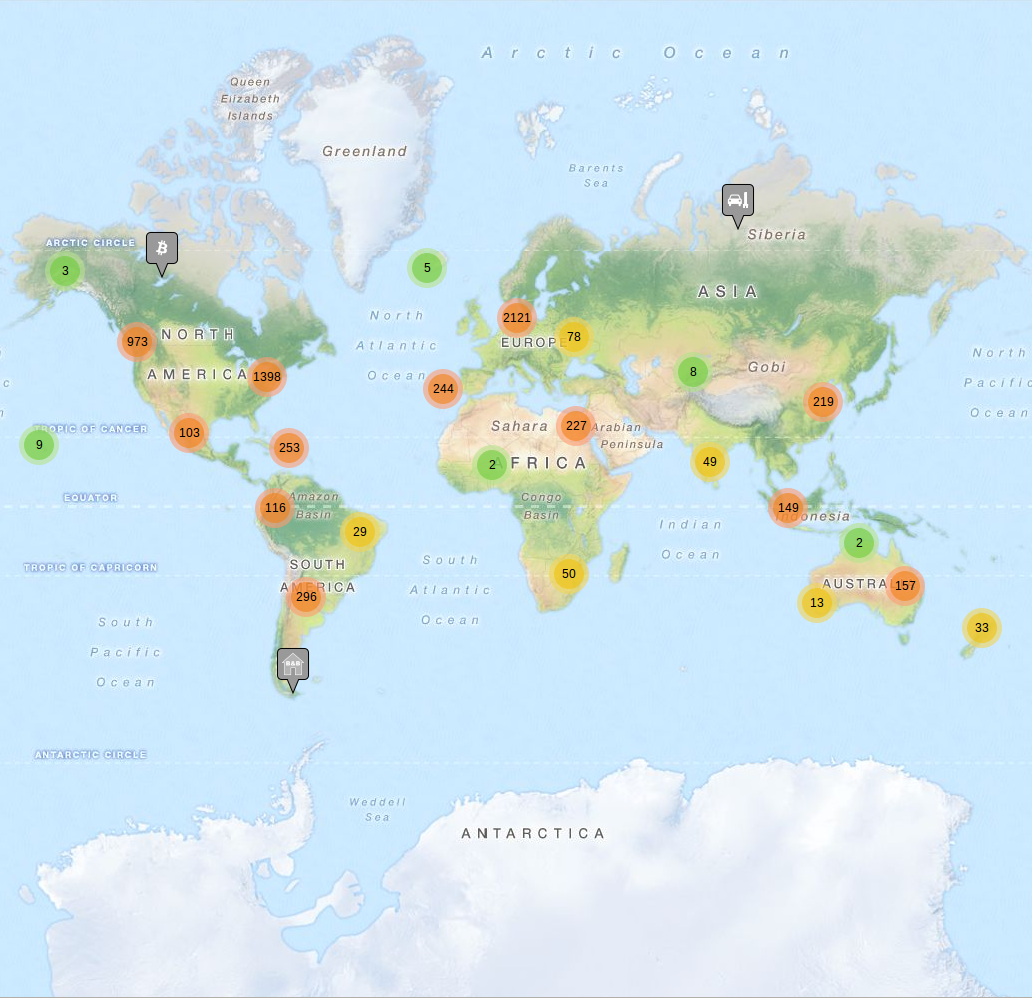
\includegraphics[width=.5\textwidth]{coinmap}
\end{frame}

%%-------------------------------------------------------------------------------------------------------------

\begin{frame}{How does one obtain Bitcoin?}
	\begin{itemize}
	\item Buy them on Exchanges, such as Bitstamp.com
	\item Offer goods or services for Bitcoin
	\item Mining (only on industrial scale today)
	\end{itemize}
\end{frame}

%%-------------------------------------------------------------------------------------------------------------

\begin{frame}{Is Bitcoin anonymous?}
No. Bitcoin is private, but completely transparent. Therefore, it is not anonymous per se, but rather pseudonymous.

Strategies to maintain privacy in the network:
\begin{itemize}
	\item Use every address only once, i.e. especially don't get your salary always paid to the same address.
	\item Don't spend transaction outputs together from accounts that should not be linked.
\end{itemize}

Nodes don't have identities. Addresses can be changed frequently, mining is performed almost independently of either of those.
\end{frame}

%%-------------------------------------------------------------------------------------------------------------

\begin{frame}{Identity in the Bitcoin Network}
\begin{itemize}
	\item Addresses stand in as \emph{Identities} in the Bitcoin network.
	\item Only the owner can speak for the identity as only the owner of the secret key can validly sign messages
\end{itemize}
\end{frame}

%%-------------------------------------------------------------------------------------------------------------

\begin{frame}{Why is it easy to verify blocks, but hard to find them?}
\begin{itemize}
	\item To find a block one has to find a combination of the block content and a random value which maps to a subset of the possible hashoutputs
\end{itemize}
\end{frame}

%%-------------------------------------------------------------------------------------------------------------

\begin{frame}{Double-Spending}
	Double-Spending: How do you know that you are the sole owner of a digital good? I.e. images are easy to copy and distribute. The problem is to create a distributed consensus.

	Bitcoin solves the Double-Spending problem. This happens by publishing updates to the balances in the network through a blockchain. The blockchain is immutable, because it is secured by Proof of Work.
\end{frame}

%%-------------------------------------------------------------------------------------------------------------

\begin{frame}{What is a Cryptographic Hashfunction?}
\end{frame}

%%-------------------------------------------------------------------------------------------------------------

\begin{frame}{How does Bitcoin achieve decentralization?}
Who maintains the ledger?
Who has authority over transaction validity?
Who creates new bitcoins?
Who determines changes in the rules of the Bitcoin systems?
Why are Bitcoins valuable?

\end{frame}

%%-------------------------------------------------------------------------------------------------------------

\begin{frame}{Distributed Consensus}
	\begin{block}{Goal}
	When the protocol terminates, all correct nodes decide on the same value.	
	\end{block}
	
	\begin{block}{Challenges}
	\begin{itemize}
		\item Malicious Nodes
		\item Latency and no "global time"
		\item Byzantine generals problem
		\item not all nodes interconnected / online at all times
	\end{itemize}
	\end{block}

	\begin{block}{Solution}
		Embraces randomness\\
		Incentivizes good behavior
	\end{block}
\end{frame}

\backupend
\end{document}
